\documentclass[12pt]{article}
\usepackage[a4paper,top=1.05cm,bottom=1.0cm,left=0.9cm,right=0.9cm]{geometry}
\usepackage[utf8]{inputenc}
\usepackage[T1]{fontenc}
\usepackage[spanish,es-nodecimaldot]{babel}
\usepackage{lmodern}
\usepackage{helvet}
\renewcommand{\familydefault}{\sfdefault}
\usepackage{graphicx}
\usepackage{hyperref}
\usepackage{multicol}
\usepackage[most]{tcolorbox}
\usepackage{fancyhdr}
\usepackage{enumitem}
\usepackage{xcolor}
\usepackage{microtype}

\graphicspath{{diagramas/}{gráficos/}{graficos/}{../resultados/gráficos/}{../resultados/diagramas/}}
\pagestyle{fancy}
\fancyhf{}
\fancyfoot[C]{\scriptsize Documento elaborado con inteligencia artificial (GitHub Copilot en modo agente) para el curso IIC103G.}
\renewcommand{\headrulewidth}{0pt}
\renewcommand{\footrulewidth}{0pt}
\setlength{\headheight}{0pt}
\setlength{\headsep}{0pt}
\setlength{\footskip}{14pt}
\setlength{\columnsep}{0.42cm}
\setlength{\parindent}{0pt}
\setlength{\parskip}{1pt}
\setlist[itemize]{leftmargin=1.0em,itemsep=0pt,topsep=1pt,parsep=0pt}
\hypersetup{hidelinks}
\definecolor{navy}{HTML}{17324D}
\definecolor{blue}{HTML}{2F6690}
\definecolor{pale}{HTML}{EDF4F8}
\definecolor{amber}{HTML}{F5C26B}
\definecolor{grey}{HTML}{ECEFF2}

\tcbset{
  colback=white,
  colframe=navy,
  arc=1.5mm,
  boxrule=0.6pt,
  boxsep=2pt,
  left=2mm,right=2mm,top=2pt,bottom=2pt,
  before skip=4pt,after skip=4pt
}

\begin{document}
\begin{tcolorbox}[colback=navy,colframe=navy,before skip=0pt,after skip=4pt]
\centering
\color{white}
{\fontsize{19}{21}\selectfont\bfseries Congestión vehicular: CMTD no homogéneas}\\[-1mm]
{\fontsize{13}{15}\selectfont Modelos estocásticos para decisiones semafóricas}\\[0.5mm]
{\bfseries Tesis: la dinámica y la persistencia cambian por hora, clima y tipo de día.}
\end{tcolorbox}

\begin{tcolorbox}[colback=pale,colframe=blue,title=\bfseries Contexto y tesis]
\textbf{Problema:} evaluar si $X_n\in\{\mathrm{Low},\mathrm{Moderate},\mathrm{High},\mathrm{Severe}\}$
sigue una CMTD no homogénea dependiente del régimen $r$ (hora, clima, día).
\textbf{Datos:} $204.000$ observaciones; $100$ intersecciones; $20$ variables; $0$ nulos;
7 días y distintos climas.
\end{tcolorbox}

\begin{multicols}{2}
\begin{tcolorbox}[title=\bfseries Recuadro 1. Formulación estocástica y arquitectura]
\begin{center}
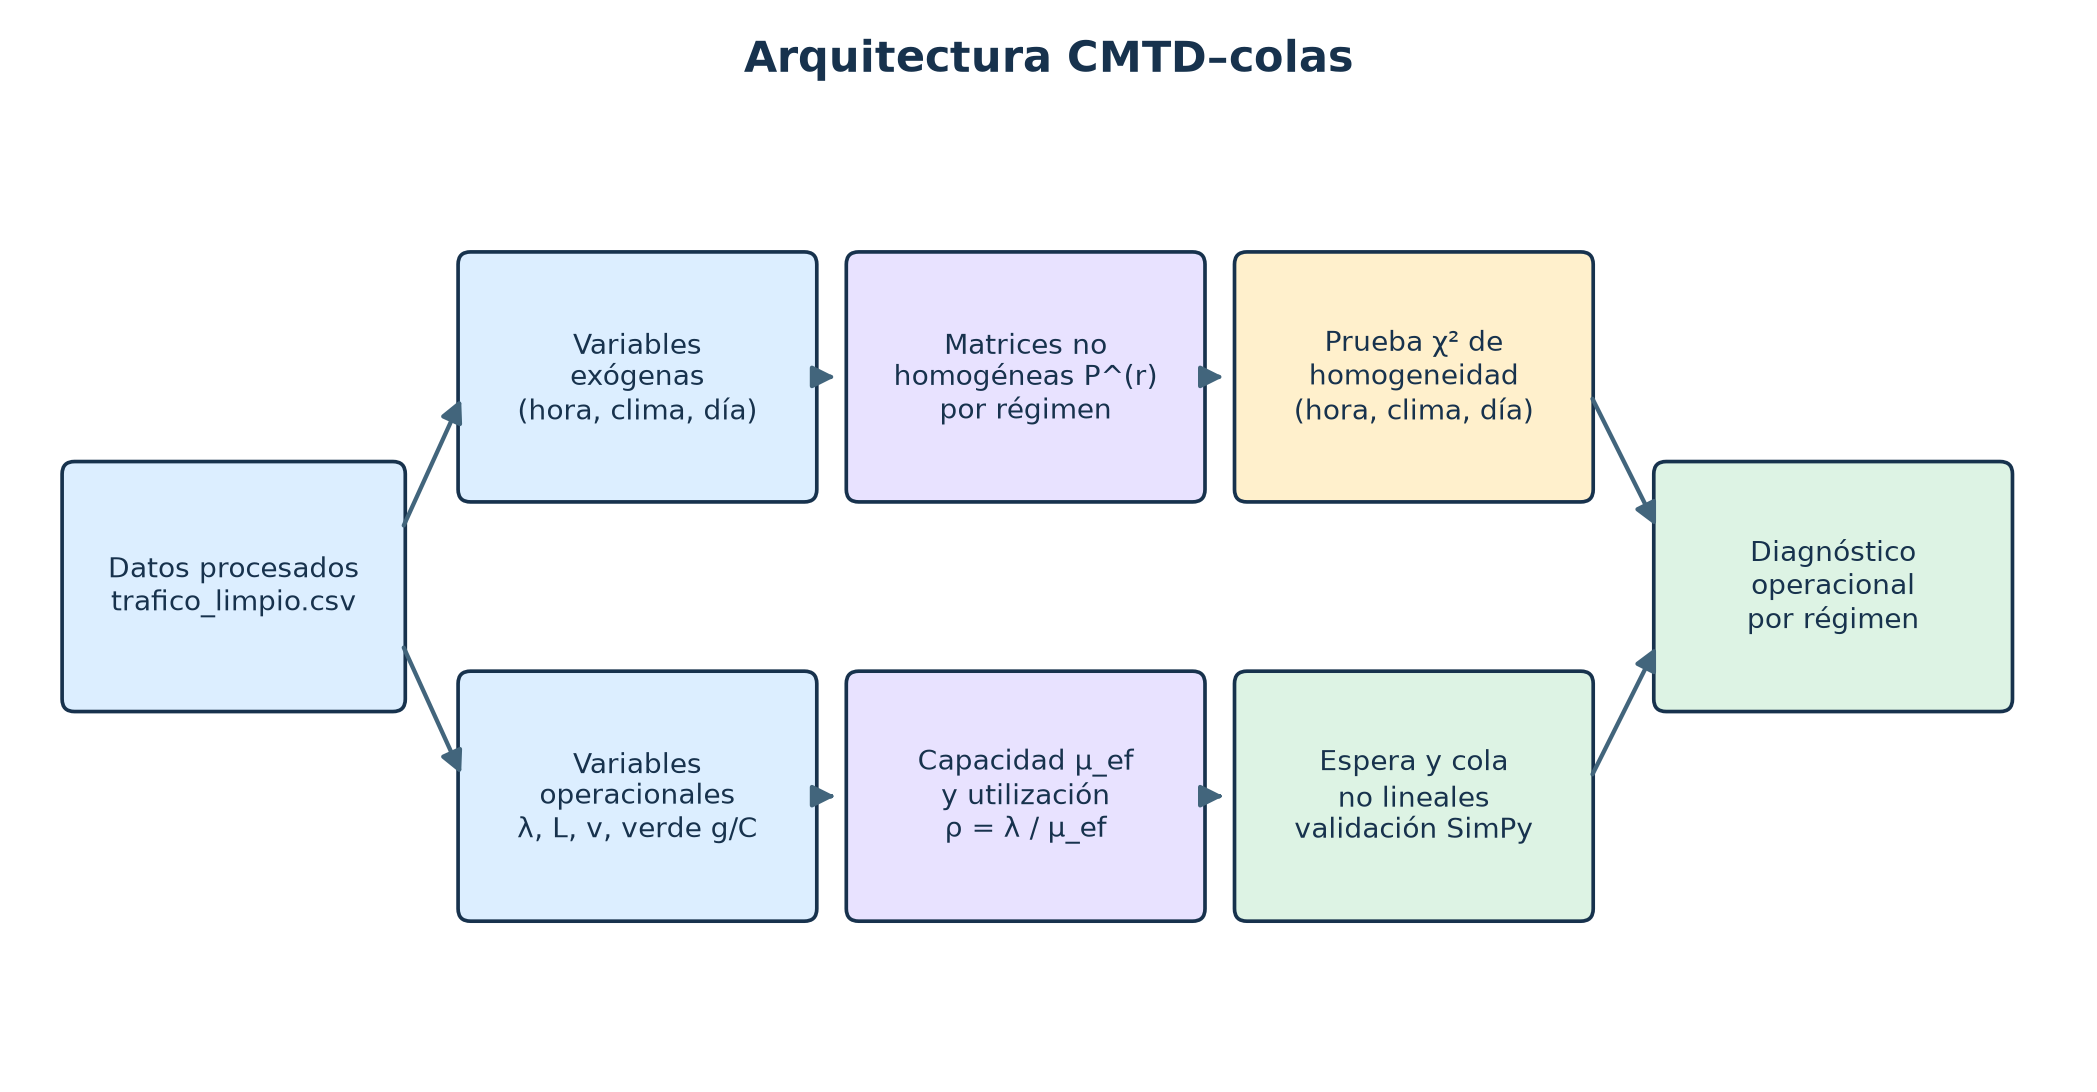
\includegraphics[width=\linewidth,height=3.6cm,keepaspectratio]{diagrama_2_arquitectura_modelo.png}
\end{center}
\textbf{Transiciones:}
$\widehat P_{ij}^{(r)}=N_{ij}^{(r)}/\sum_kN_{ik}^{(r)}$ por régimen.
\textbf{Colas:} $\rho=\lambda/\mu_{\mathrm{ef}}$, con $\lambda$ observada y $\mu_{\mathrm{ef}}$
determinada por pistas, velocidad y $g/C$.
\end{tcolorbox}

\begin{tcolorbox}[title=\bfseries Recuadro 2. No homogeneidad de $P^{(r)}$]
\textbf{Contraste extremo:}
\textit{Night | Clear}: $P_{\mathrm{Low,Low}}=0,976$.
\textit{Evening Peak | Rain}: $P_{\mathrm{Severe,Severe}}=0,128$.
\begin{center}
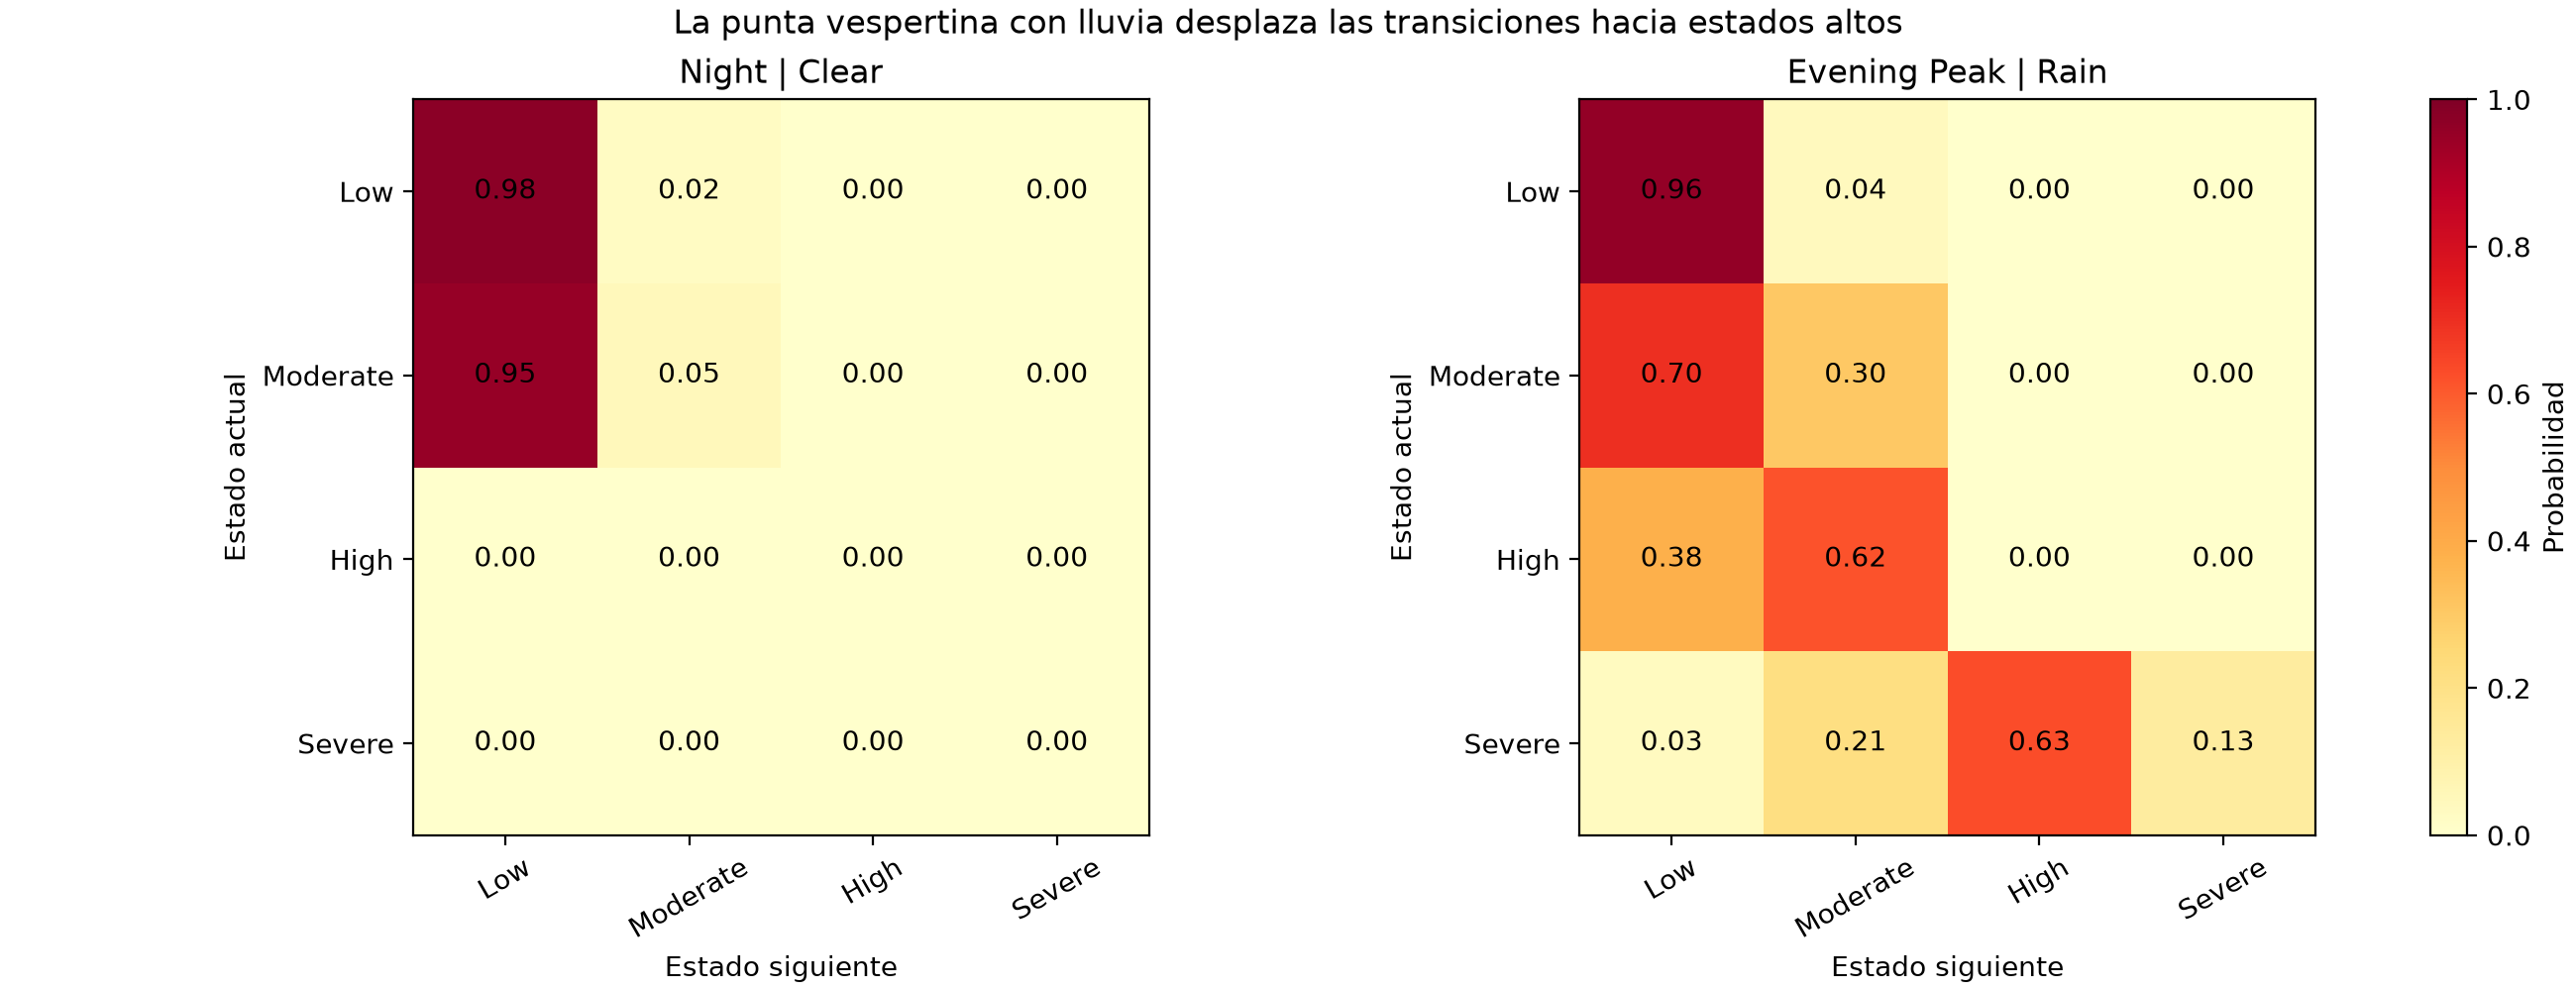
\includegraphics[width=\linewidth,height=3.6cm,keepaspectratio]{heatmap_transiciones.png}
\end{center}
\textbf{Pruebas:} homogeneidad rechazada por franja, clima y tipo de día
($p<0,001$ en cada contraste).
\end{tcolorbox}
\end{multicols}

\noindent
\begin{minipage}[t]{0.58\linewidth}
\begin{tcolorbox}[colback=grey,colframe=navy,title=\bfseries Recuadro 3. Distribución empírica $\pi^{(h)}$]
\begin{center}
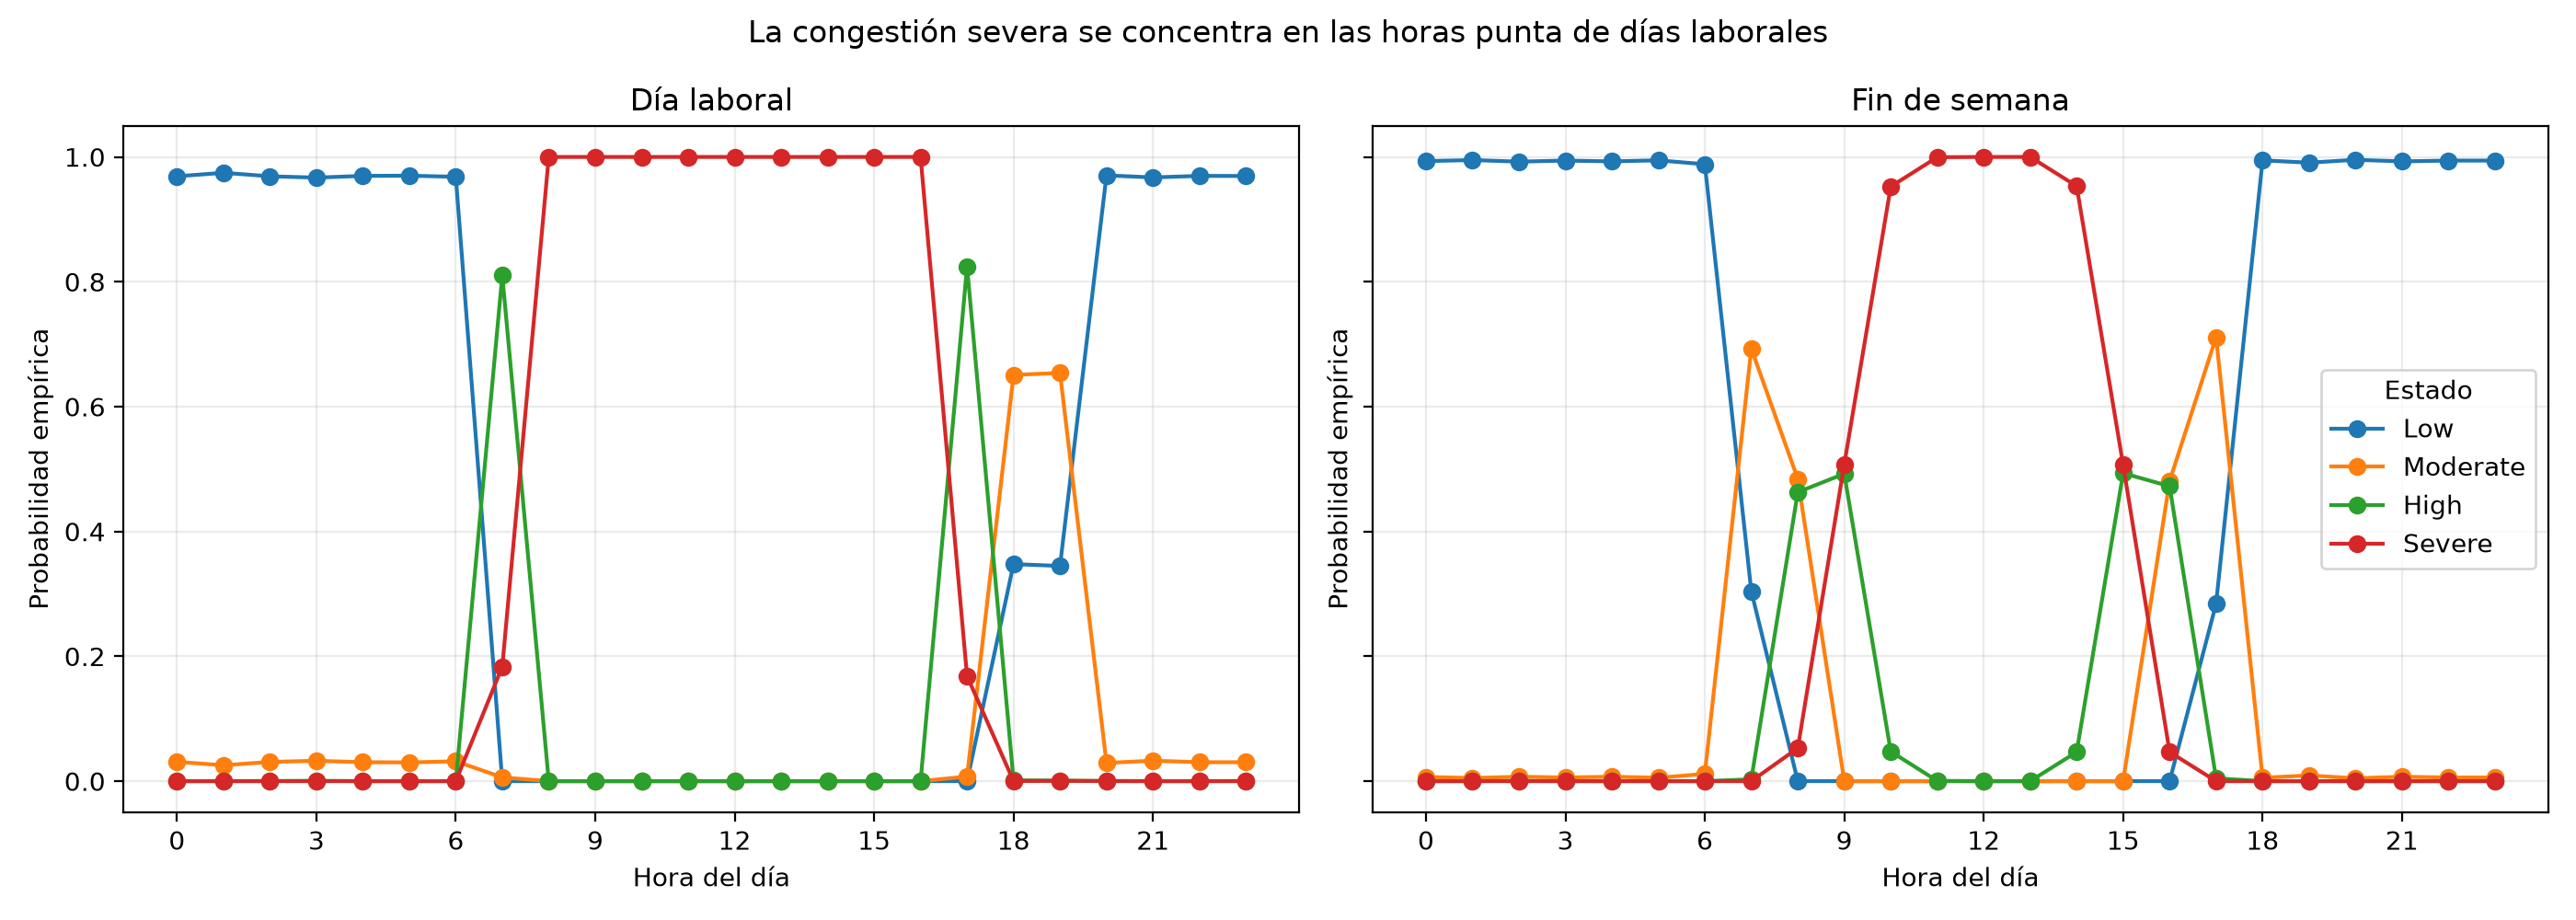
\includegraphics[width=\linewidth,height=3.4cm,keepaspectratio]{evolucion_horaria_estados.png}
\end{center}
\textbf{Lectura:} las curvas muestran
$\widehat{\mathbb P}(X_n=i\mid h)$; las cuatro suman $100\%$.
En horas punta laborales, reflejan el efecto acumulado de
$\pi^{(h+1)}=\pi^{(h)}P^{(r)}$.
\end{tcolorbox}
\end{minipage}\hfill
\begin{minipage}[t]{0.38\linewidth}
\begin{tcolorbox}[colback=amber!28,colframe=amber!90!black,title=\bfseries Conclusiones y límites]
\begin{itemize}
\item Una matriz única subestima persistencia en estados altos.
\item El crecimiento no lineal cerca de $\rho\to1$ alcanza $R^2=0,4223$ y es consistente con SimPy.
\item Resultados observacionales: calibrar $\mu_{\mathrm{ef}}$ con aforos en terreno para inferencia causal.
\end{itemize}
\end{tcolorbox}
\end{minipage}

\end{document}
